\section{El juego del Go}
\label{sec:juego_go}
El Go es un juego de mesa estratégico muy popular en Asia.
En él, dos jugadores colocan alternativamente fichas negras y blancas (llamadas \textbf{piedras})  sobre las intersecciones libres de un tablero de dimensiones 19$\times$19.
El objetivo del juego es controlar una porción más grande del tablero que el oponente.

Existen versiones del juego en tableros más pequeños (9$\times$9, 13$\times$13 ó 17$\times$17).
El tamaño más común es 19$\times$19 y es el que se usa en los torneos oficiales \citeref{InternationalGoFederation, EuropeanGoFederation}.
Aquí se ha considerado una versión generalizada del juego en un tablero de dimensiones \textit{N$\times$N}.

\bigskip
A continuación se exponen las reglas del juego, basadas en las \textit{``Reglas Tromp/Taylor''} (más conocidas como \textit{``Reglas lógicas del Go''}) que tienen las características de ser muy elegantes y concisas \citeref{reglasLogicas}.

\subsection{Reglas del juego}
\label{ssec:reglas_go}
Al inicio de la partida el tablero está vacío y se juega con $N \times N$ piedras blancas y $N \times N+1$ negras, donde $N \times N$ son las dimensiones del tablero (180 piedras blancas y 181 negras para un tablero 19$\times$19).
El jugador con las piedras negras juega primero. 
Después ambos jugadores mueven por turnos.
Un movimiento consiste en poner una piedra en una intersección vacía del tablero o bien pasar el turno. Si ambos jugadores pasan el turno consecutivamente, la partida termina.

Dos o más piedras juntas (horizontal o verticalmente) del mismo color forman un \textbf{grupo}.
Las \textbf{libertades} de una piedra o grupo son las intersecciones vacías horizontales o verticales, adyacentes a esa piedra o grupo. 
Una piedra sola en el medio del tablero tiene cuatro libertades, una piedra en el borde tiene tres libertades y una piedra en la esquina tiene dos.

Una piedra o grupo de piedras se captura y retira del tablero de juego si no tiene libertades, esto es, si se encuentra completamente rodeada de piedras del color contrario.
Las piedras capturadas no pueden volver a jugarse durante la partida.

En principio está permitido jugar en cualquier punto del tablero (incluidos los bordes y las esquinas), pero existen dos movimientos prohibidos: el \textbf{suicidio} y la \textbf{situación de \textit{Ko}}.
\begin{itemize}
	\item \textbf{Suicidio} \\
	Está prohibido ubicar una piedra en una posición que no captura ninguna otra y deja a su propia piedra o grupo sin libertades. En la figura~\ref{fig:go_suicidio} se aprecia esta situación, mientras que la figura~\ref{fig:go_no_suicidio} no representa una situación de suicidio.
\begin{figure}[t]
	\centering
	% Primera imagen
	\begin{minipage}[t]{0.4\linewidth}
		\centering
		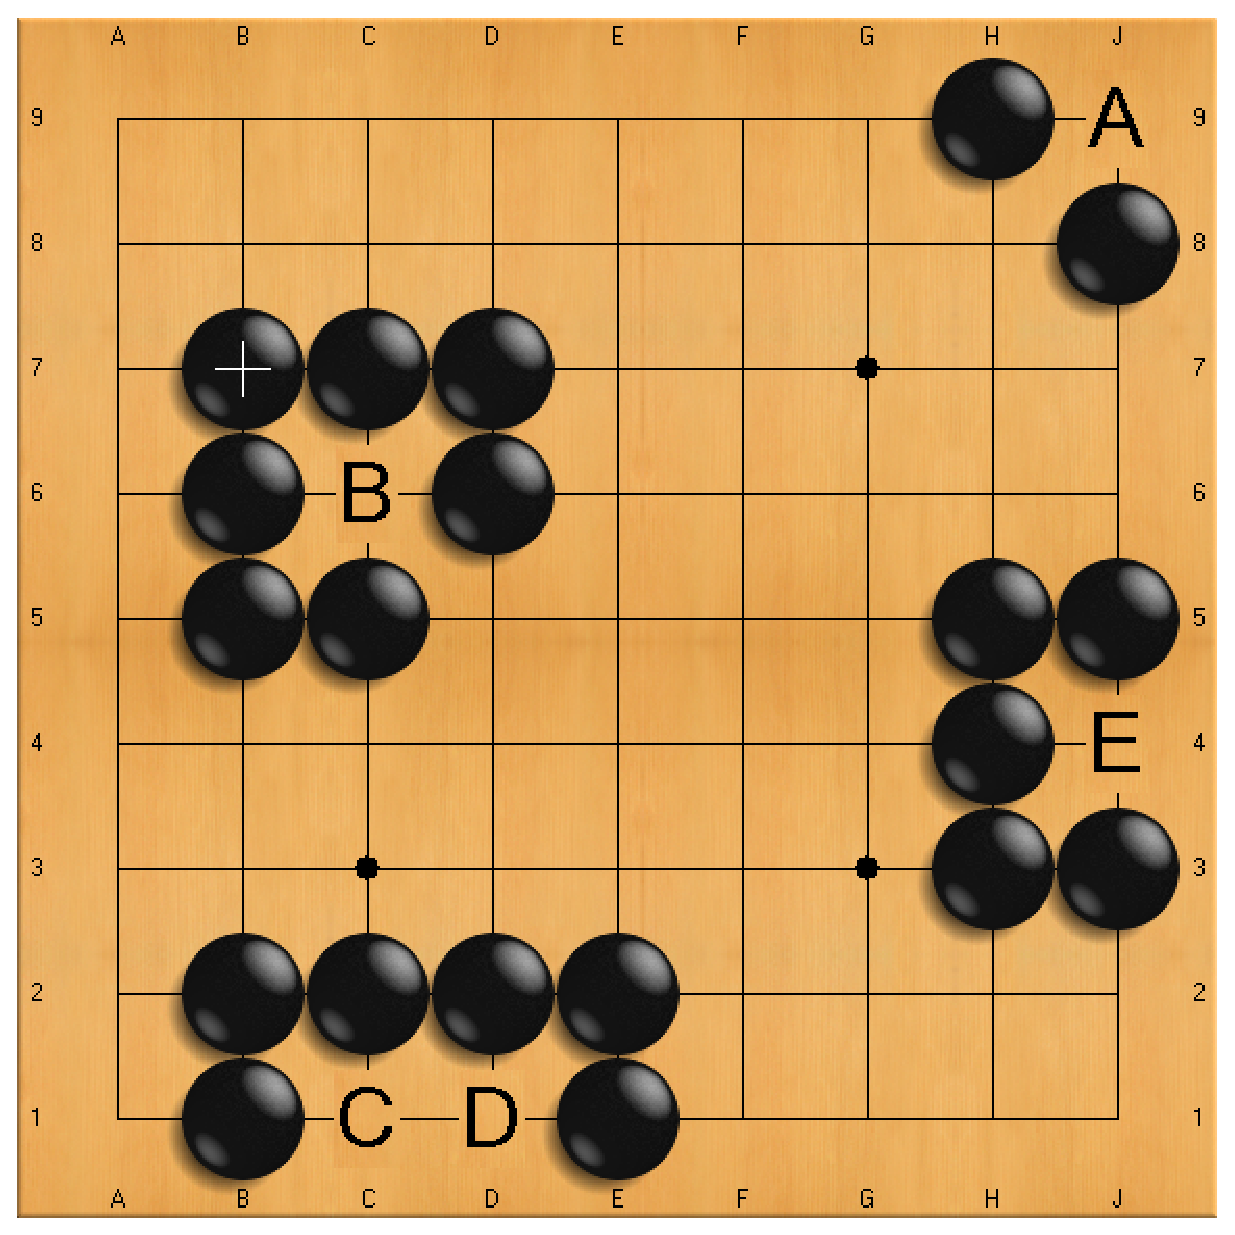
\includegraphics[scale=0.2]{contenido/cap2/imagenes/suicidio.eps}
		\caption[Situación de suicidio en el Go]{Situación de suicidio. Blancas no pueden mover en A, B o E.}
		\label{fig:go_suicidio}
	\end{minipage}
	\hspace{1cm}
	% Segunda imagen
	\begin{minipage}[t]{0.4\linewidth}
		\centering
		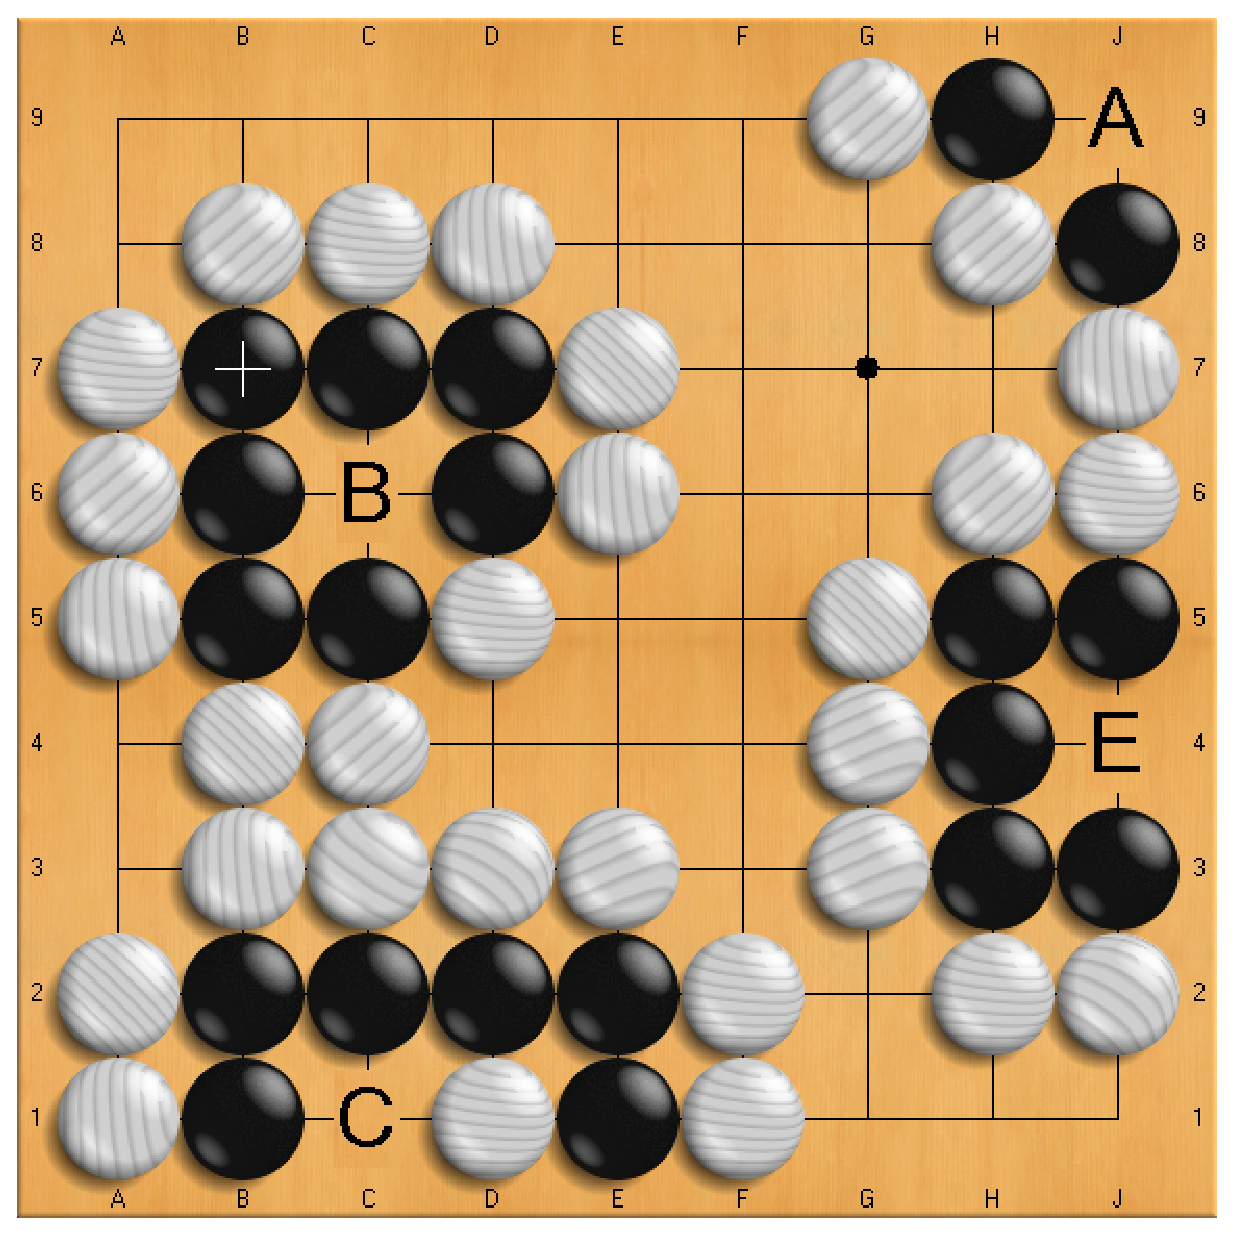
\includegraphics[scale=0.2]{contenido/cap2/imagenes/no_suicidio.eps}
		\caption[Situación de captura en el Go]{Blancas pueden mover en A, B, C o E, pues ha rodeado completamente al enemigo.}
		\label{fig:go_no_suicidio}
	\end{minipage}
\end{figure}
	\item \textbf{La regla del \textit{Ko}} \\
	La regla del \textit{Ko} evita que las posiciones de las piedras en el tablero se repitan en dos turnos diferentes.
Los tableros de la figura~\ref{fig:go_ko} reflejan esta situación.
Si un jugador captura una piedra en situación de \textit{Ko}, otro jugador no puede recapturar la misma piedra inmediatamente; ha de hacer otra jugada antes de recapturar.
Se trata de evitar una situación de infinitud.
\begin{figure}[t]
	\centering
	% Primera imagen
	\begin{minipage}[t]{0.4\linewidth}
		\centering
		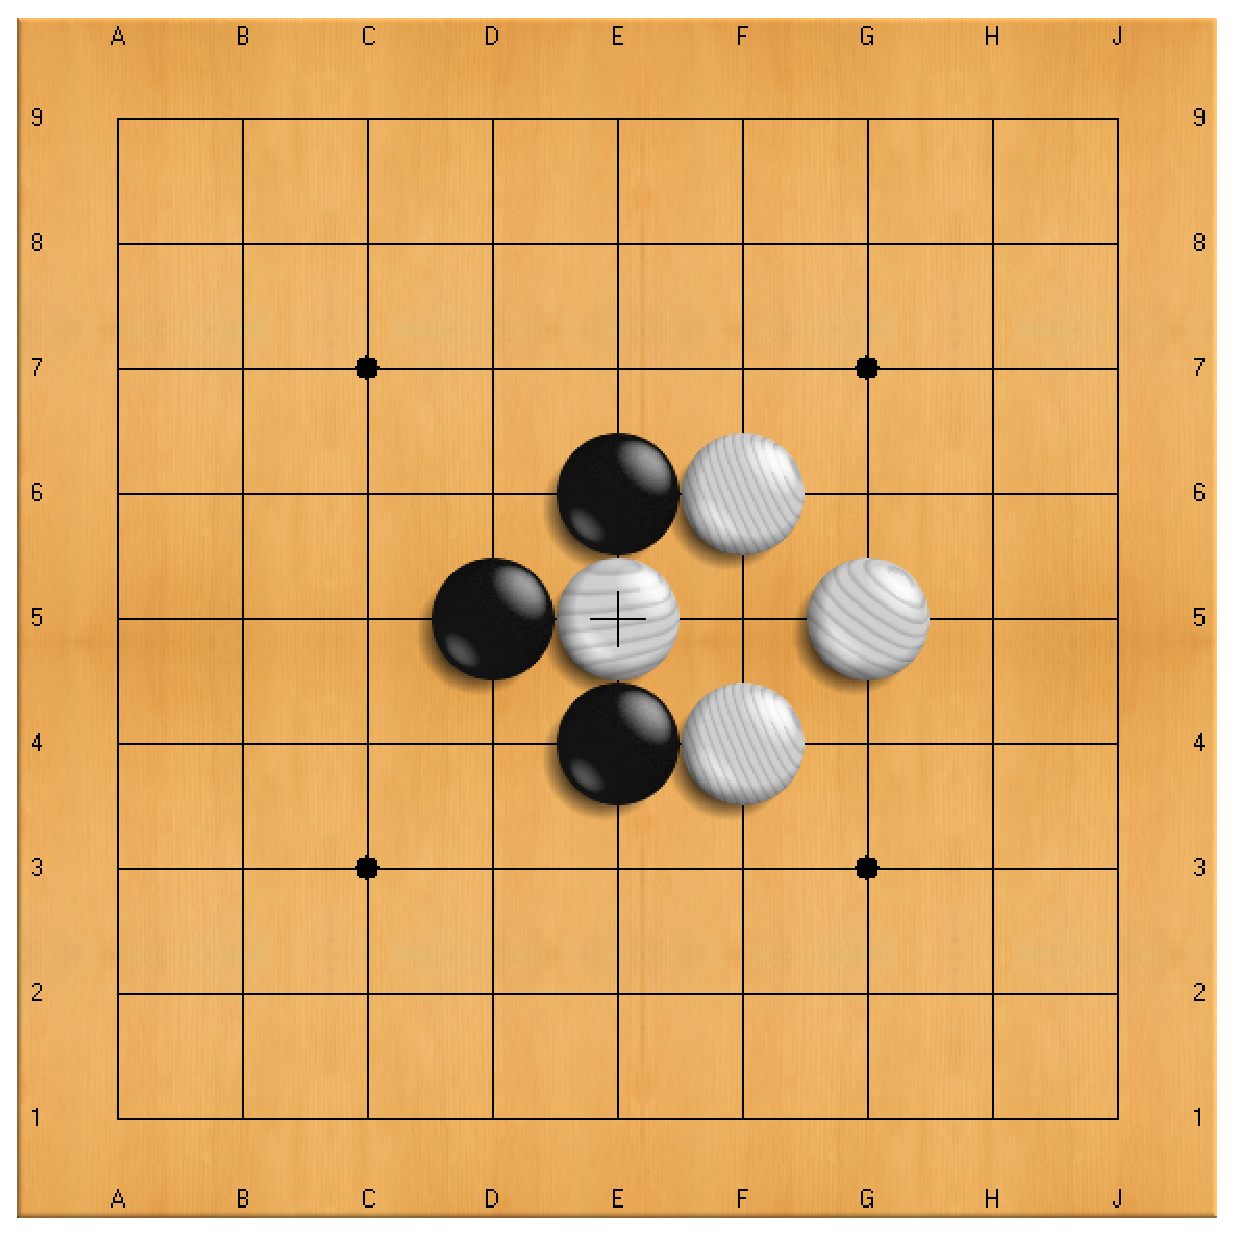
\includegraphics[scale=0.2]{contenido/cap2/imagenes/ko1.eps}
	\end{minipage}
	\hspace{1cm}
	% Segunda imagen
	\begin{minipage}[t]{0.4\linewidth}
		\centering
		\includegraphics[scale=0.2]{contenido/cap2/imagenes/ko2.eps}
	\end{minipage}
	\caption[Situación de \textit{Ko} en el Go]{Situación de \textit{Ko}.}
	\label{fig:go_ko}
\end{figure}
\end{itemize}

Una partida de Go termina cuando ambos jugadores consideran que ya no existen territorios por disputar.
Cuando esto ocurre ambos jugadores pasan turno consecutivamente.
En una partida profesional, tal circunstancia la decide un juez.
Una partida también puede terminar si ambos jugadores han agotado sus piedras.

El \textbf{territorio} está formado por las intersecciones del tablero que se encuentren vacías.
El \textbf{territorio privado} está formado por las intersecciones que se encuentran dentro de algún cerco de uno u otro jugador.
El \textbf{territorio público} es aquel que no está cercado por ninguno de los jugadores y no influye en la puntuación final.
Hay ciertos territorios conquistados que no se encuentran protegidos del todo, pero que si el jugador contrario los atacase perdería de todas formas, luego son parte del territorio privado de quien lo tiene cercado.

El ganador de la partida es el jugador con más puntos.

\subsubsection{Puntuación}
\label{sssec:puntuacion_go}
Existen dos formas de contar los puntos de una partida: según las reglas japonesas y según las reglas chinas:

\bigskip

\begin{itemize}
	\item \textbf{Reglas japonesas}\\
	Cada jugador recibe un punto por cada intersección vacía dentro de su territorio, menos un punto por cada piedra que haya capturado el enemigo.
	\item \textbf{Reglas chinas}\\
	Cada jugador recibe un punto por cada intersección vacía dentro de su territorio, más un punto por cada piedra que tenga sobre el tablero. 
\end{itemize}
Ambos métodos producen el mismo resultado. Las reglas de puntuación japonesas son las más extendidas y son las que se usan en los torneos oficiales.

El jugador con piedras negras tiene ventaja debido a que siempre mueve primero.
Para compensar esta ventaja se suma una cantidad de puntos al jugador blanco.
A estos puntos se les denomina \textit{komi} y son determinados antes de empezar la partida.
El valor de \textit{komi} puede variar según los distintos reglamentos; suele oscilar entre 5.5 y 7.5 puntos para un tablero 19x19.
Este valor también es usado para evitar que una partida termine en empate.

\subsubsection{\textit{Handicap}}
\label{ssec:handicap_go}
En el Go existe un sistema de \textit{handicap} o ventaja para igualar una partida entre jugadores de diferente nivel.

El \textit{handicap} consiste en un número de piedras colocadas sobre el tablero antes de empezar la partida.
En ese caso el jugador de menor nivel jugará con las piedras negras y comenzará con un número determinado de piedras ya colocadas sobre el tablero.
Estas piedras se colocan sobre los puntos marcados del tablero, quedando las piedras de forma simétrica.
También existen otras variantes de \textit{handicap} libre, en el cual el jugador coloca las piedras de ventaja donde él quiera.

El número de piedras de \textit{handicap} depende de la diferencia de nivel entre los jugadores. 
Existe una clasificación oficial de niveles para los jugadores de Go \citeref{MCTS2}.
